%=========================================================

% Here you can choose to compile with or without solutions.
% However, this definition is ignored if you use any
% command from the `Makefile`.
\providecommand{\withSol}{\iftrue}

%=========================================================

\documentclass
[twoside,german,colorbacktitle,accentcolor=tud9c]
{tudexercise}

\usepackage[T1]{fontenc}
\usepackage[utf8]{inputenc}
\usepackage[ngerman]{babel}
\usepackage{amstext}
\usepackage{amsmath}
\usepackage{graphicx}
%\usepackage{setspace}
\usepackage{multicol}
\usepackage{mathtools}
\usepackage{dsfont}
\usepackage{units}
%\usepackage{subfigure}
\usepackage{color}
\usepackage{booktabs}
\usepackage{fancyref}
\usepackage{gensymb}
\usepackage{tikz}
\usetikzlibrary{shapes.misc} 
\usepackage[verbose]{placeins}%Floatbarrier
\tikzset{root/.style={align=center,draw=none},level 2/.style={align=center,left=1.5cm}}


%=========================================================


\setcounter{section}{6}
%=========================================================

\newcommand{\grp}{F}

%=========================================================


\begin{document}

\title{GDV 2 -- Theorie Übung \arabic{section}}
\subtitle{Sommer Semester 2019}
\subsubtitle{Übungsgruppe \grp{}}

\maketitle

%=========================================================



\begin{examheader}
	\textmb{GDV 2 - Theorie Übung \arabic{section} | Gruppe \grp{}}\\
	\begin{tabular}{l l l l l}
		Moritz Fuchs	& Alexander Jäger	& Amon Ditzinger	& John Kalkhof	\\
	\end{tabular}
\end{examheader} 


%=========================================================
% Anpassung an Aufgabenstellung
\renewcommand\thesubsection{Aufgabe \arabic{subsection}}
\renewcommand\thesubsubsection{\alph{subsubsection})}

%=========================================================
\FloatBarrier
\newif\ifvimbug
\vimbugfalse

\ifvimbug
\begin{document}
\fi


\subsection{Euler-Formeln (7 Punkte)}
\subsubsection{2 Punkte}
\subsubsection{2 Punkte}
\subsubsection{3 Punkte}
\newif\ifvimbug
\vimbugfalse

\ifvimbug
\begin{document}
\fi


\subsection{Netzkompression (8 Punkte)}
\subsubsection{2 Punkte}
\subsubsection{3 Punkte}
\subsubsection{3 Punkte}
\newif\ifvimbug
\vimbugfalse

\ifvimbug
\begin{document}
\fi


\subsection{Punktwolken (6 Punkte)}
\subsubsection{0.5 Punkte}
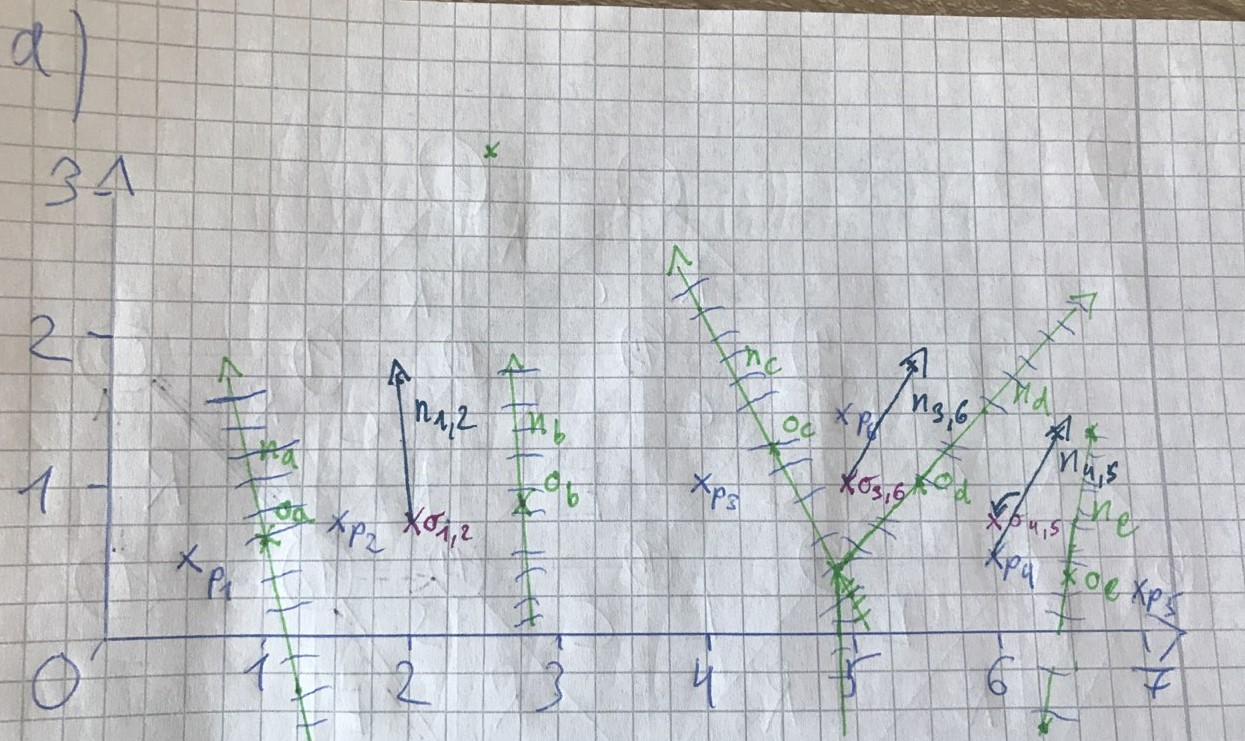
\includegraphics[scale=0.5]{3b.jpg}
\subsubsection{1 Punkt}
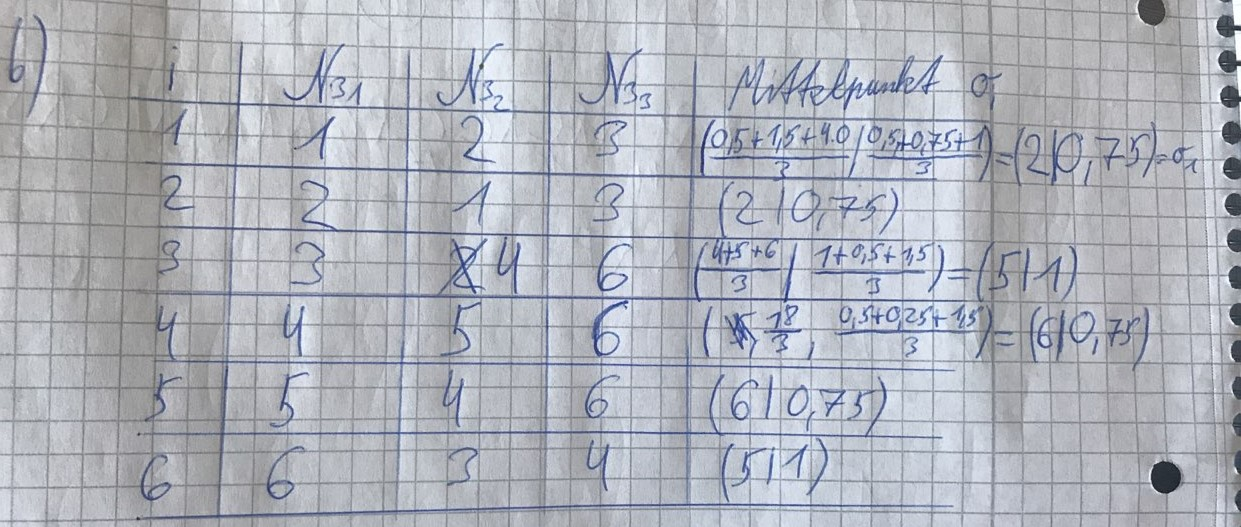
\includegraphics[scale=0.5]{3c.jpg}\\
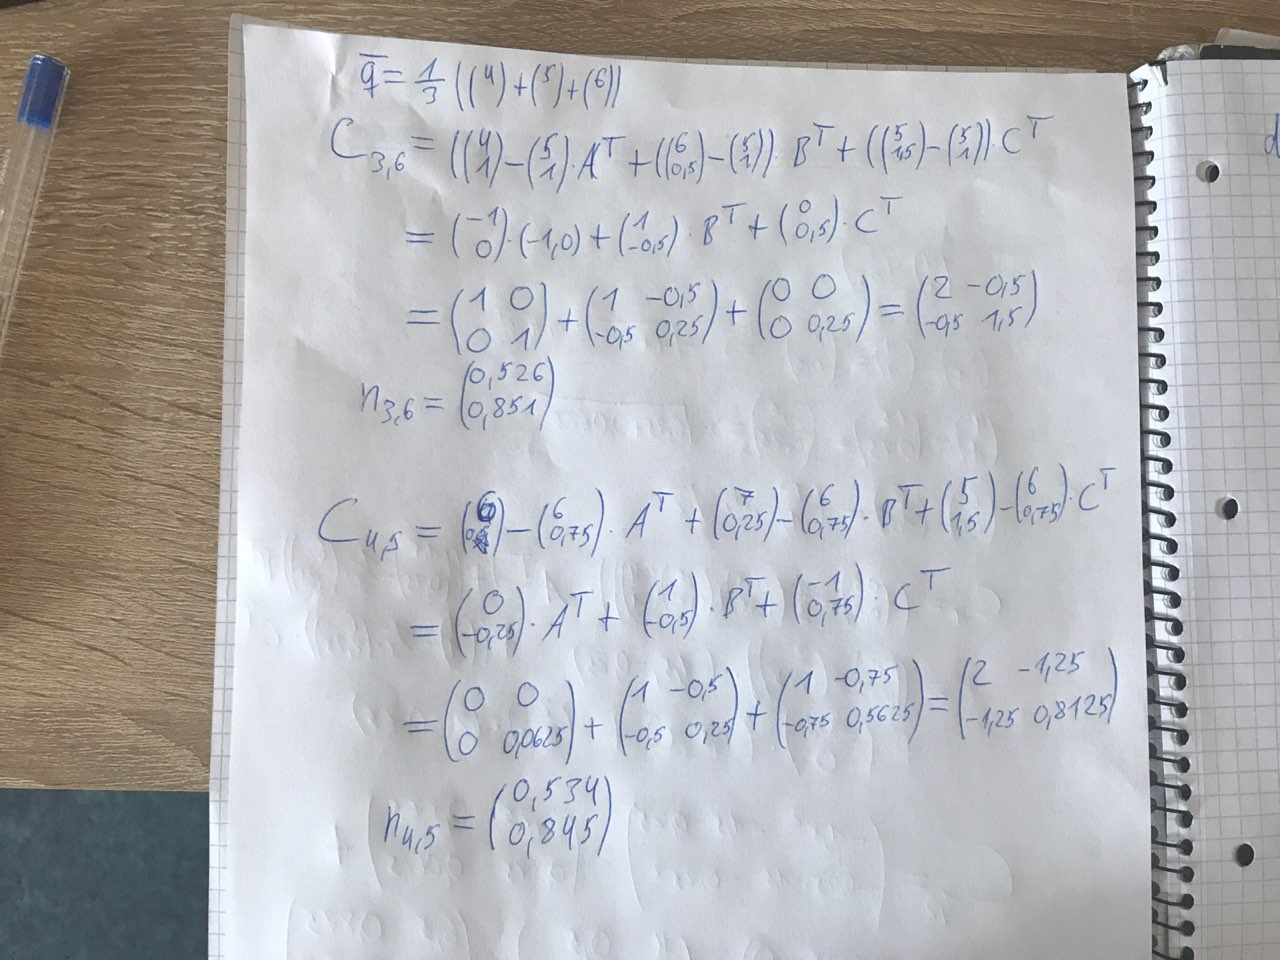
\includegraphics[scale=0.3]{3bR.jpg}\\
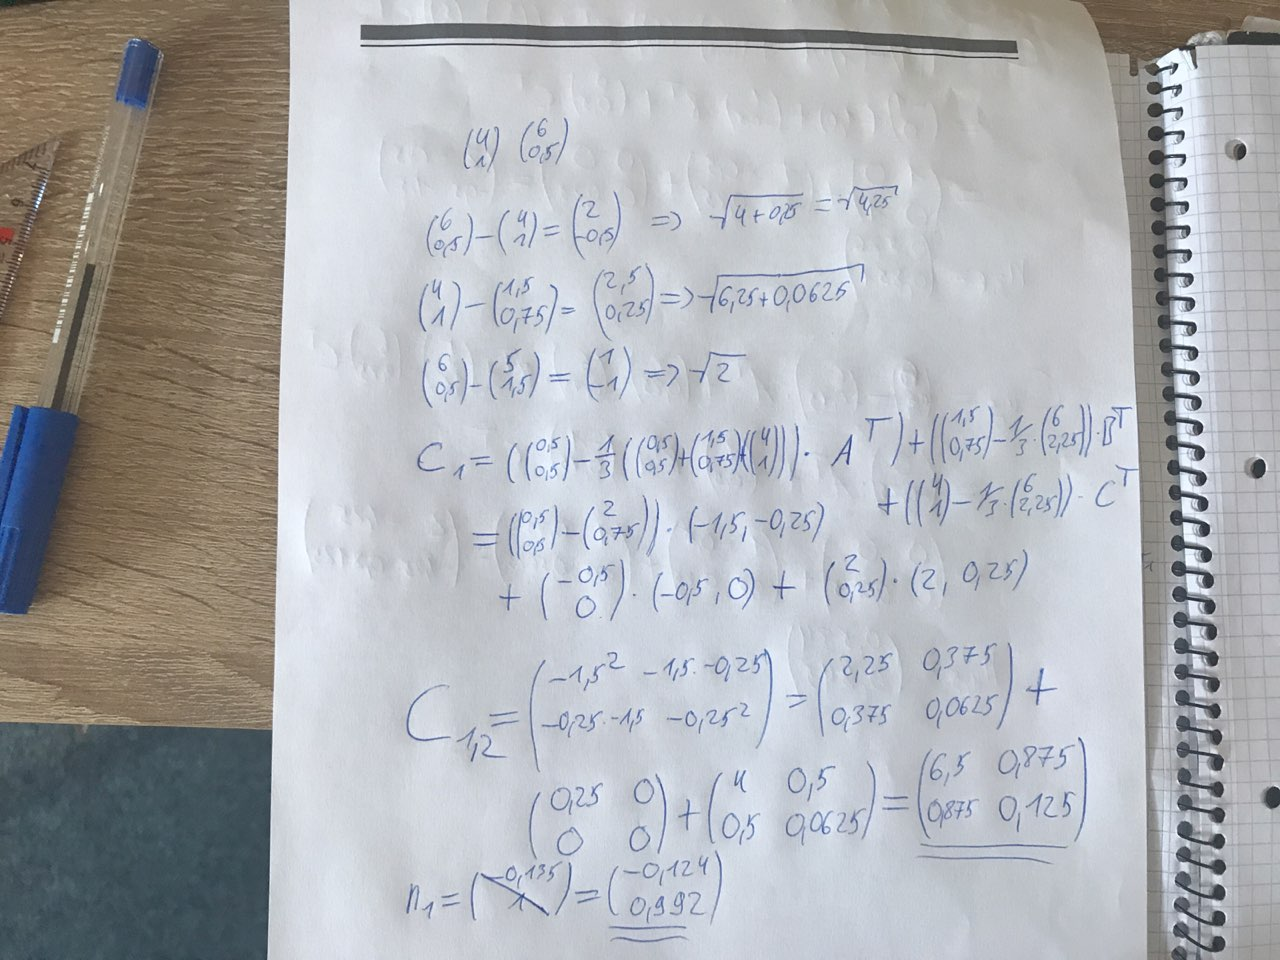
\includegraphics[scale=0.3]{3bR2.jpg}
\subsubsection{1.5 Punkte}
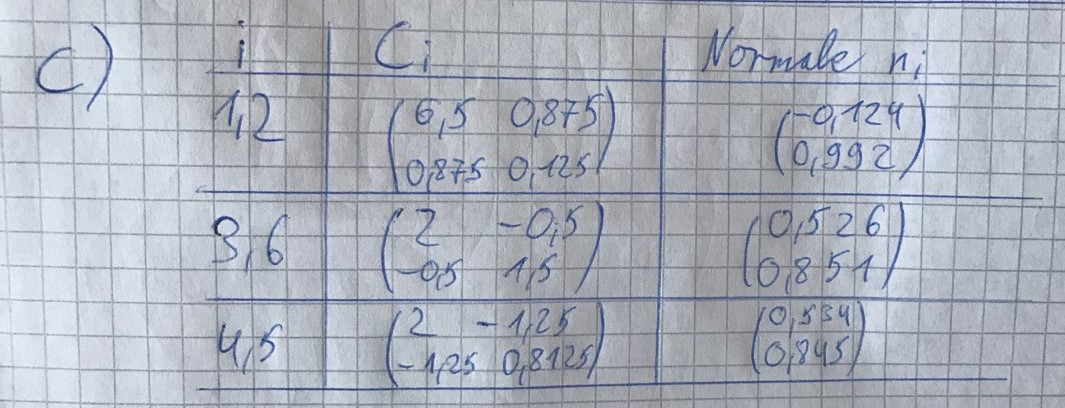
\includegraphics[scale=0.5]{3d.jpg}
\subsubsection{0.5 Punkte}
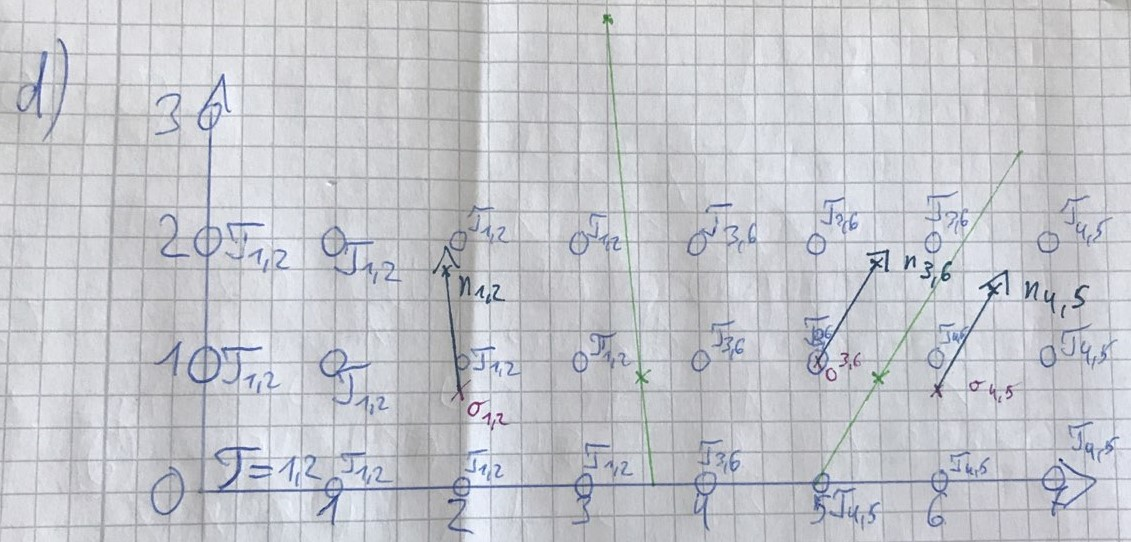
\includegraphics[scale=0.5]{3a.jpg}
\subsubsection{1.5 Punkte}
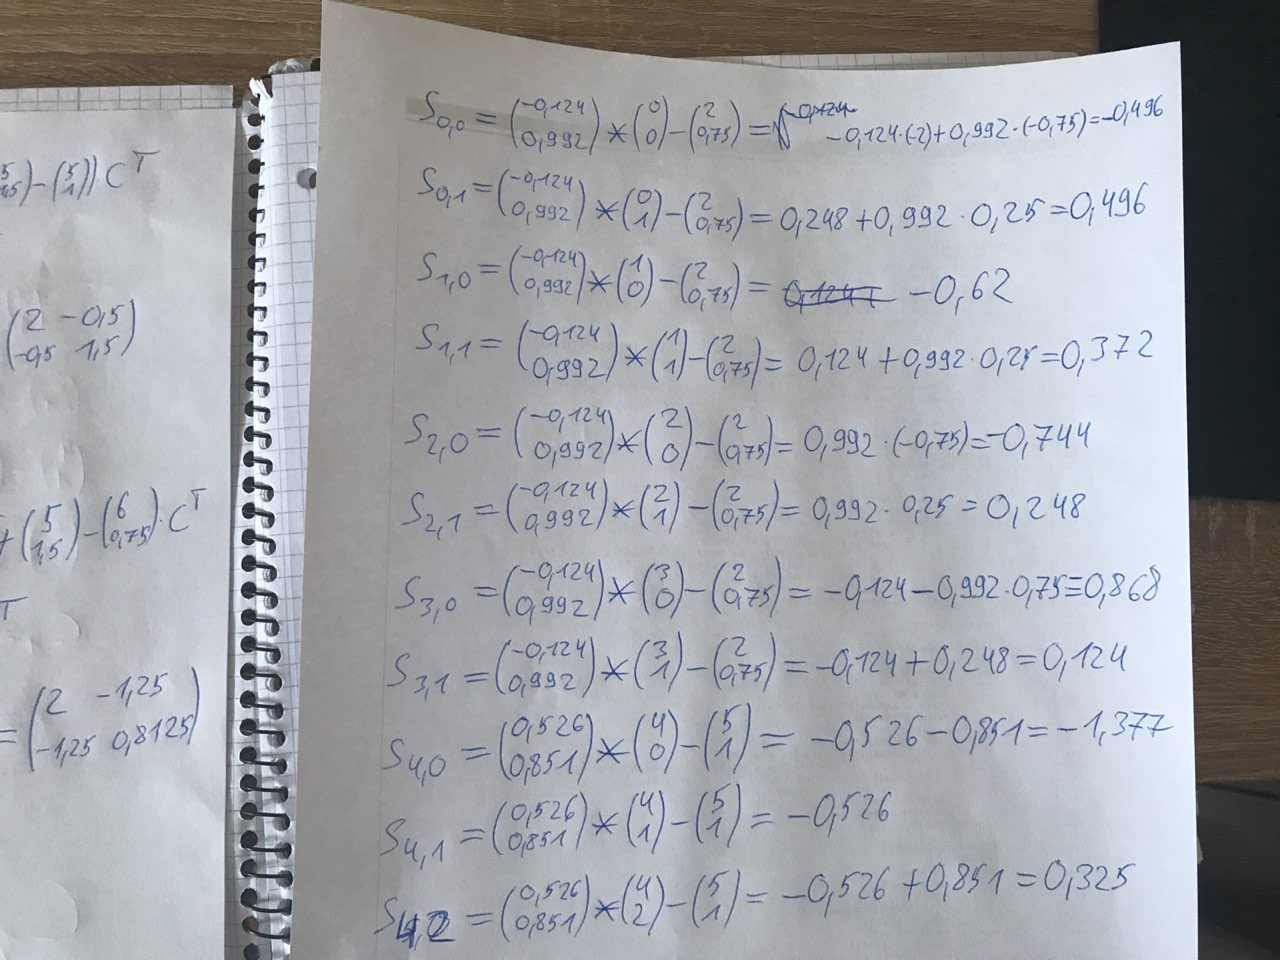
\includegraphics[scale=0.3]{3dR.jpg}
\subsubsection{1 Punkt}



%=========================================================

\end{document}
